\chapter{Introducere}

%Aceasta lucrare își propune sa prezinte, din punct de vedere atât teoretic cat și practic în ce consta dezvoltarea unui algoritm de recunoaștere a obiectelor în imagini, folosind tehnici de procesare a imaginilor și învățare automata.

Prin intermediul acestei lucrări doresc să prezint, din punct de vedere teoretic, pașii necesari în dezvoltarea unui sistem de recunoaștere a obiectelor în imagini, folosind tehnici de procesare a imaginilor și învățare automată.

Totodată, această lucrare vine însoțită de implementarea unei biblioteci software pentru dezvoltarea de algoritmi și aplicații de recunoaștere a obiectelor.
În plus, pe baza acestei biblioteci, am implementat unul dintre algoritmii de recunoaștere consacrați.



\section{Motivație}

Recunoașterea obiectelor este una dintre principalele aplicații ale viziunii artificiale și procesarea de imagini. 

Oamenii pot recunoaște o mulțime de obiecte într-o imagine fără sa depună prea mult efort, chiar dacă în aceste imagini obiectele prezintă variații de perspectiva, de dimensiune, sunt translatate, rotite sau chiar obstrucționate. 
Cu toate că de-a lungul timpului au fost studiați și dezvoltați multi algoritmi, sistemele de recunoaștere automată a obiectelor sunt încă departe de performanta unei ființe umane, chiar de cea a unui copil de numai doi ani.
Așadar, încă există loc pentru cercetarea și dezvoltarea algoritmilor în acest domeniu.

%În ciuda performantei relativ scăzute a acestor algoritmi, odată cu dezvoltarea sistemelor hardware, fapt ce a permis aplicarea unor algoritmi mult mai complicați sau au putut fi aplicați pe niște probleme de dimensiune mai mare, cererea de aplicații a crescut. 

Odată cu dezvoltarea sistemelor hardware, fapt ce a permis aplicarea unor algoritmi mult mai complicați sau a făcut posibilă aplicarea celor deja existenți pe niște probleme de dimensiune mult mai mare, cererea de aplicații a crescut.
Câteva dintre cele mai de succes aplicații sunt: 
\begin{itemize}
	\item Sistemul de frânare automată la detecția pietonilor instalat pe mașinile Volvo.\cite{volvo}
	\begin{figure}[H]
		\centering
			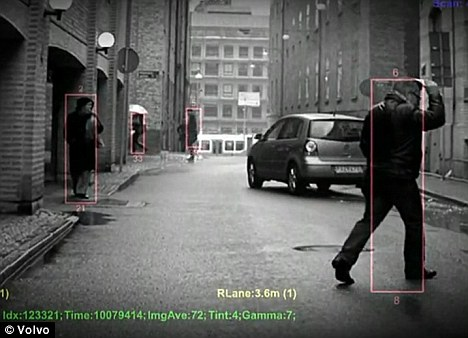
\includegraphics[width=0.8\textwidth]{imagini/volvo_pedestrian_detection.jpg}
		\caption{Volvo: sistemul de detecție a pietonilor\cite{VolvoArticle}}.
		\label{fig:volvo_pedestrian_detection}
	\end{figure}
	
	\item Focalizarea automată a camerelor foto pe fețe		
	\begin{figure}[H]
		\centering
			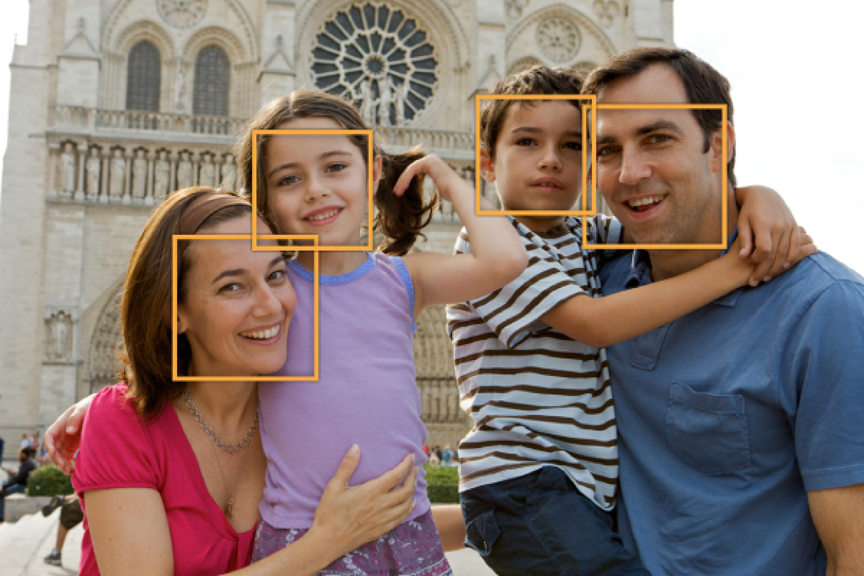
\includegraphics[width=0.8\textwidth]{imagini/face_detection_2x.png}
		\caption{Cameră foto: focus automat\cite{CanonFaceRecognition}}
		\label{fig:face_detection_2x}
	\end{figure}
	


	\item Analizarea traficului rutier	
	\begin{figure}[H]
		\centering
			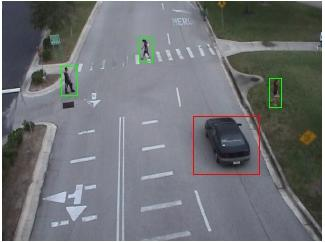
\includegraphics[width=0.9\textwidth]{imagini/traffic_analisys.jpg}
		\caption{Analizarea traficului rutier\protect\footnotemark}
		\label{fig:traffic_analisys}
	\end{figure}

\end{itemize}
	\footnotetext{\url{http://youtu.be/PXSiUojhNFg}}

Înțelegerea și dezvoltarea unui sistem de recunoaștere automată a obiectelor poate fi foarte dificilă, mai ales pentru cei care sunt la început de drum în studierea acestui domeniu. 
Documentația de specialitate, de cele mai multe ori, este scrisă privind problema de la un nivel foarte înalt și nu sunt tratate detaliile algoritmilor. 
În același timp, în foarte multe lucrări se fac referiri la lucrări anterioare, unele chiar cu zeci de ani distantă intre ele, acestea fiind uneori foarte greu de găsit.
Parcurgerea unui astfel de document presupune cunoștințe extensive de matematică, statistică, învățare automată, procesarea imaginilor și chiar cunoștințe din domeniul biologic sau medical. 
Toate acestea fac ca nivelul de la care se intră acest domeniu sa fie unul foarte înalt, ceea ce poate fi descurajant pentru un începător.

Exista câteva biblioteci software bune, "open-source", cu care se pot dezvolta aplicații: 
opencv\footnote{\url{http://opencv.org/}}, 
dlib\footnote{\url{http://dlib.net/}}, 
libccv\footnote{\url{http://libccv.org/}}.
Avantajele lor sunt:
\begin{itemize}
	\item Există algoritmi de recunoaștere a obiectelor gata implementați.
	\item Se poate trece direct la dezvoltarea de aplicații
\end{itemize}
Totuși sunt și dezavantaje:
\begin{itemize}
	\item Componentele care stau la baza acestor implementări nu sunt expuse, reutilizarea lor fiind imposibilă.
	\item Codul sursă este optimizat cu instrucțiuni de asamblare sau pentru procesorul grafic, fiind dificil de înțeles.
\end{itemize}
Aceste dezavantaje fac ca aceste biblioteci sa nu fie utile celor care doresc sa dezvolte sau să studieze astfel de algoritmi.

La finalul lucrării s-a obținut o platformă de dezvoltare a algoritmilor pentru recunoașterea obiectelor, pe care să o pot folosi în activitatea mea din domeniu și care să servească drept punct de plecare pentru cei care doresc să se inițieze în domeniu.

Avantajele acestei platforme ar fi:
\begin{itemize}
	\item Fiecare componentă a unui algoritm de recunoaștere este implementat într-o clasă separată
	\item Algoritmii pot fi implementați atât în C++ cât și în Python
	\item Reutilizare sporită a componentelor
	\item Pot fi ușor adaptați algoritmi din alte biblioteci pentru utilizare în cadrul platformei
\end{itemize}

C++ și Python sunt două limbaje de programare foarte diferite, dar tocmai aceste diferențe fac ca cele două să se îmbine aproape perfect, formând un mediu de lucru prielnic studierii și dezvoltării de algoritmi.

%Viziunea artificiala reprezinta procesul invers al celui de formare a imagini și se ocupa cu recuperarea de informații din imagini cu ajutorul metodelor matematice, geometrice, statistice și a teoriei învățării automate\footnote{Machine learning}.

%Recunoașterea automata a obiectelor se refera la capacitatea unui sistem software de localizare și identificare a obiectelor într-o imagine sau o secventa video.

%Din punct de vedere practic, aceasta lucrare își propune dezvoltarea unei biblioteci software și aplicații demonstrative, cu ajutorul cărora sa se poată dezvolta aplicații de recunoașterea obiectelor în imagini.

%Din punct de vedere teoretic sunt descrise componentele și structura unui astfel algoritm, precum și cel folosit pentru al antrena.



%Viziunea artificiala și învățarea automata sunt doua domenii aflate în plina dezvoltare și sunt de mare interes atât în cadrul academic ca și în industria software.

%Dezvoltarea rapida a sistemelor de calcul a permis utilizarea acestor algoritmi în tot mai multe aplicații. Câteva dintre aplicațiile recunoașterii de obiecte sunt:
%\begin{itemize}
%	\item Industriale: recunoașterea și verificarea cip-urilor pe o placa electronica, numărarea de obiecte pe o banda rulanta
%	\item Securitate: recunoașterea unui intrus folosind o camera de supraveghere
%	\item Medicale: recunoașterea diferitelor tumori într-o imagine de tomografie
%	\item Fotografie: focalizare automata pe fete
%	\item Internet: căutare google după imagini, marcarea automata a fetelor într-o poza de pe facebook
%\end{itemize}

%Interesul 

%Pana acum am folosit și am studiat o mulțime de algoritmi de recunoaștere a obiectelor, dar pentru a aprofunda înțelegerea acestor algoritmi cel mai bine este sa fie scris măcar unul de la un capăt la altul.

%Cei mai multi algoritmi de recunoaștere a obiectelor au o structura comuna formata din următoarele componente: scanarea imaginii, extragerea de trasaturi, classificare si procesarea rezultatelor.

%Multi algoritmi sunt scrisi intr-un mod foarte rigid si componentele lor nu pot fi refolosite. Sunt optimizati pana la punctul in care codul sursa nu mai poate fi inteles cu usurinta.

%In cadrul companiei la care lucrez, Dynamic Ventures, am folosi

%Desi, am folosit si m-am documentat 

%Am ales sa dezvolt o astfel de librarie, chiar daca exista si altele, din doua motive.





%Aceasta problema nu poate fi nici pe departe considerata rezolvata, de-a lungul timpului un număr mare de algoritmi au fost propuși.

%Mult timp recunoașterea automata a obiectelor în imagini a fost considera impracticabila datorita complexității de timp și spațiu a acestor algoritmi.






\section{Enunțul problemei}
Se scrie o bibliotecă software cu ajutorul căreia să se dezvolte algoritmi și aplicații de recunoaștere a obiectelor.

Această bibliotecă va fi scrisă într-un mod hibrid, cu componente implementate atât în C++ cât și în Python.
Această combinație de limbaje va permite implementarea rapidă a algoritmilor în Python, iar la nevoie aceștia pot fi implementați parțial în C++.

Toate componentele bibliotecii vor suporta serializare pentru a putea fi salvate pe disc, baze de date sau trimise prin rețea în cazul unor programe distribuite.
De asemenea se serializează rezultatul unor sesiuni lungi de antrenare.

Algoritmul va învăța sa recunoască obiecte folosindu-se de un set de imagini cu exemple pozitive adnotate și exemple negative, imagini care nu conțin obiectul pe care dorim sa-l învățam.
Algoritmul poate fi personalizat prin alegerea de implementări diferite ale componentelor de către utilizator.

Ca exemplificare, se scrie o aplicație care antrenează un algoritm de recunoaștere și salvează modelul învățat pe disc și o altă aplicație care încarcă modelul și îl aplică pe o imagine data.



\section{Structura Lucrării}


Capitolele care urmează vor trata algoritmii de recunoaștere a obiectelor din punct de vedere teoretic și se va prezenta implementarea unei platforme de dezvoltare a acestora.

În capitolul 2 sunt prezentate în detaliu structura algoritmilor de recunoaștere și o tehnică eficienta de antrenare.

În capitolul 3 sunt prezentate tehnologiile folosite.

În capitolul 4 sunt prezentate în detaliu structura cadrului de lucru, implementarea unui algoritm de recunoaștere și modalități de extindere a bibliotecii.

În capitolul 5 sunt prezentate concluzii despre lucrare, precum și posibilități de dezvoltare.

\pagebreak